\chapter{Data Augmentation Techniques}
\label{cha:overviewOfDataAugmentation}

%---------------------------------------------------------------------------

Data augmentation is a technique used to increase the diversity of data available for training models without collecting new data. This method involves applying various transformations to existing data samples to create altered versions. This method involves making changes to existing data samples by applying various transformations such as rotations, scaling, cropping, and adjusting lighting conditions. The goal of data augmentation is to make the resulting model more robust, which reduces the likelihood of overfitting and improves its ability to generalize to new, unseen data~\cite{ImageDataAugmentationSurvey}. 

In this chapter, available methods of image augmentation are introduced and the reasons for using data augmentation are explained. The classification of augmentation methods is shown in Figure \ref{fig:augDiagram}.

\begin{figure}[!htb]
    \centering
    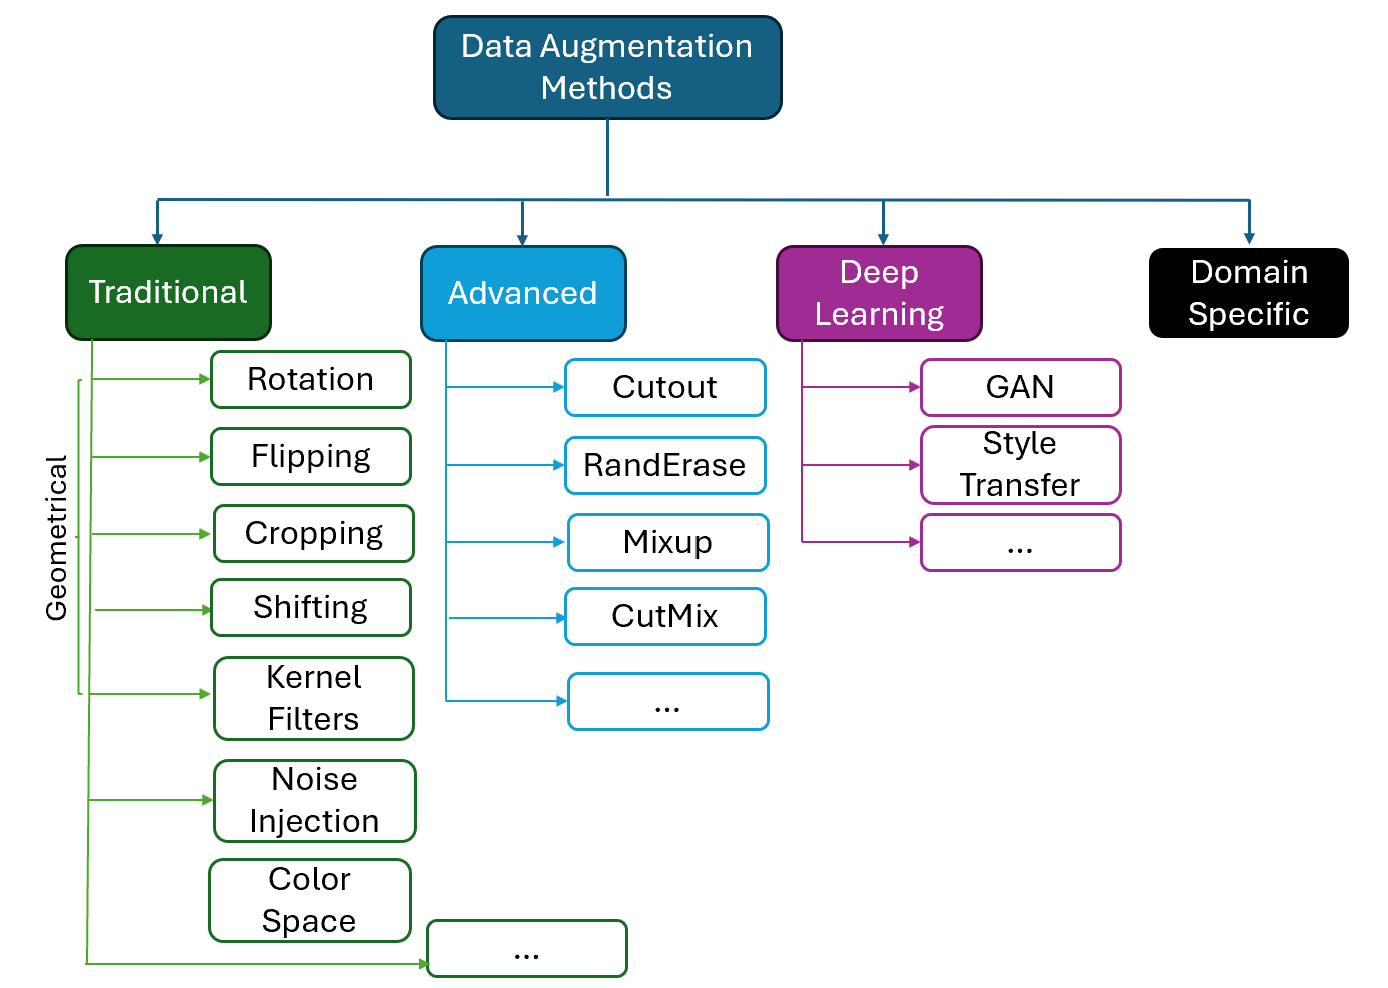
\includegraphics[scale=0.8]{Images/augmentation-diagram.png}
    \caption{Diagram showing the classification of augmentation methods. \\ Inspired by~\cite{AugmentationDiagram}.}
    \label{fig:augDiagram}
\end{figure}

\section{Why Data Augmentation is Essential}

Image data augmentation is an essential technique in the field of deep learning, particularly in tasks involving image recognition and classification. In this section, the reasons and justifications for employing image data augmentation will be explored, deriving insights from Suorong Yang's survey~\cite{DataAugmentationEssential} while integrating additional perspectives from related studies.

\textbf{Handling Overfitting}. One of the primary motivations for using image data augmentation is to reduce overfitting. Overfitting occurs when a model learns the details and noise in the training data to the extent that it negatively impacts the performance of the model on new, test data. By artificially enhancing the dataset through transformations like rotation, scaling, and flipping, the diversity within the training dataset increases. This diversity helps the model generalize better to new, unseen images, therefore improving its predictive performance.

\textbf{Enhancing the Dataset without Additional Data Collection}. Deep neural networks often require large amounts of training data to prevent overfitting. However, obtaining labeled data for real-world applications can be challenging due to its scarcity. Data collection is often a resource-intensive process, requiring significant time, effort, and sometimes financial investment, especially for tasks requiring large annotated datasets. Image data augmentation provides a cost-effective method to expand the dataset without the need for additional data collection.

\textbf{Increasing Model Robustness} Another key aspect of data augmentation is its role in increasing the robustness of models. By exposing the model to a wide range of variations in the data and deformations of objects within the images, the model learns to identify the essential features of the objects regardless of their presentation. This capability is crucial for practical applications where the conditions under which images are captured can vary widely.

The methods described in the subsequent sections are frequently combined by setting a minimal threshold, in the form of a probability, for each method to occur. This approach ensures that each augmentation technique, such as rotations, flips, or color adjustments, is applied selectively rather than uniformly across all images. By doing so, it introduces a stochastic element to the augmentation process, enhancing the diversity of the training data and preventing the model from overfitting to specific attributes of the training set.
%---------------------------------------------------------------------------

\section{Traditional Data Augmentation}
\label{ssec:augmentationTraditional}

The chapter on traditional data augmentation in Conor Shorten's article "A Survey on Image Data Augmentation for Deep Learning"~\cite{ImageDataAugmentationSurvey} provides a comprehensive overview of conventional techniques used in data augmentation to enhance the robustness and generalizability of deep learning models. This article will be used as a reference when writing this subsection of the paper.
%---------------------------------------------------------------------------

\subsection{Basic Transformations}
\label{ssec:basicTransformations}


Traditional basic data augmentation methods are foundational in training deep learning models, particularly in the field of image processing. These techniques involve simple yet effective transformations to existing images in a dataset, aiming to simulate the variability that these models will encounter in real-world scenarios. Key techniques include:


\textbf{Rotation}: involves rotating each image through various angles. This process ensures diverse orientations in the dataset, fostering the model's ability to recognize objects regardless of their rotational position. Maximum rotation degree can be defined.

\textbf{Flipping}: Images are flipped horizontally or vertically. 

\textbf{Random Cropping}: Parts of images are cropped and resized to their original dimensions, teaching the model to focus on different parts of an image. A crop size smaller than the original is defined, and during training, a random starting point is selected to extract a sub-section of the image. This exposes the model to diverse sections of the image, leading to better performance.

\textbf{Shifting}: This technique involves translating the contents of an image in the horizontal or vertical direction to avoid positional bias. This manipulation simulates the effect of objects being located in different parts of the image frame, which can be crucial in tasks where object-varying localization is key.

\textbf{Kernel Filters}: Kernel filters are widely utilized in image processing to sharpen or blur images. These filters apply an n × n matrix over an image using a Gaussian blur filter to create a softer appearance or a vertical or horizontal high-contrast edge filter to enhance sharpness, particularly along edges. Using blurring in data augmentation can increase a model's tolerance to motion blur when deployed. Similarly, sharpening during data augmentation can help highlight finer details in objects.

\textbf{Noise injection}: This technique involves adding random noise (typically Gaussian) to images to mimic real-world imperfections. It helps to build noise-robust models and prevent misclassification of real-world test data, especially if the training dataset consists only of perfect images.

\textbf{Color space}: Changing color helps in training models to be invariant to color changes. Techniques such as adjusting brightness, contrast, saturation, and hue are commonly used. A simple color augmentation technique can rely on isolating one channel R, G, or B and adding two zero matrices

\begin{figure}[!htb]
    \centering
    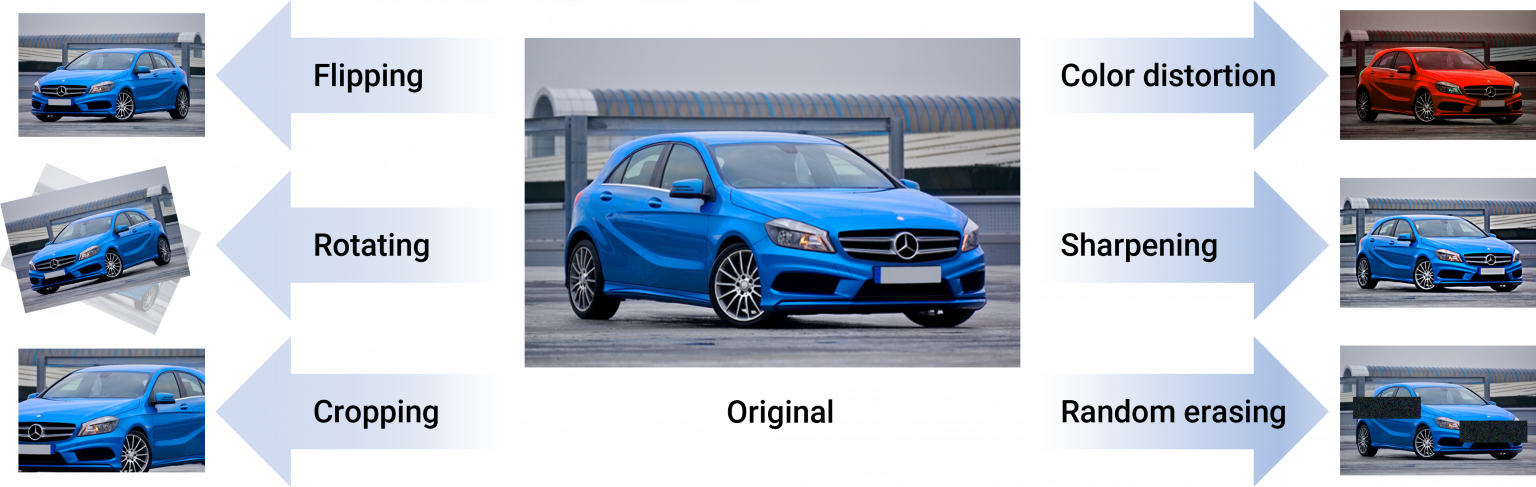
\includegraphics[scale=0.38]{Images/traditional-augmentation-examples.png}
    \caption{Traditional image augmentation examples~\cite{TradAugExamples}.}
    \label{fig:tradAugExamples}
\end{figure}
%---------------------------------------------------------------------------

\subsection{Advanced Transformations}
\label{ssec:advancedTransformations}
%---------------------------------------------------------------------------

\textbf{MixUp}: \textit{MixUp} is a data augmentation technique proposed by Hongyi Zhang et al.~\cite{MixupOriginal} that creates synthetic training examples by linearly combining pairs of images and their labels from the training data. Given two examples \( (x_i, y_i) \) and \( (x_j, y_j) \), the Mixup generated new example \( (\hat{x}, \hat{y}) \) is calculated as follows:
\begin{align*}
    \hat{x} &= \lambda x_i + (1-\lambda) x_j \\
    \hat{y} &= \lambda y_i + (1-\lambda) y_j
\end{align*}
where \( \lambda \) is a mixing coefficient sampled from a Beta distribution, typically \( \text{Beta}(\alpha, \alpha) \) for some \( \alpha > 0 \). By creating virtual examples that blend features and labels of multiple training instances, \textit{MixUp} encourages the model to learn more invariant and robust features which leads to smoother decision boundaries, reducing the likelihood of overfitting.


\textbf{CutMix}: The \textit{CutMix} method, described in~\cite{CutMixOriginal} is a data augmentation technique similar to \textit{MixUp}, but focusing on promoting localization capabilities to improve classification performance. \textit{CutMix} involves cutting parts of images and pasting them onto other images, effectively blending the features of two different classes within a single training example. The corresponding labels are also mixed proportionally to the area of the patches.

\textbf{CutOut}: Also known as \textbf{Random Erasing}, this data augmentation technique involves randomly removing or "cutting out" one or more rectangular regions from an input image during training. This forces the neural network to focus on less dominant features, enhancing its generalization ability. By limiting access to full information, CutOut encourages the model to learn more features of objects, not only the obvious ones. For example, even when only the stem of a flower is visible, the model can still identify the flower, demonstrating its ability to recognize crucial but less prominent features. Seeing the whole flower model would probably focus on the bloom not paying attention to the stem.

\begin{figure}[!htb]
    \centering
    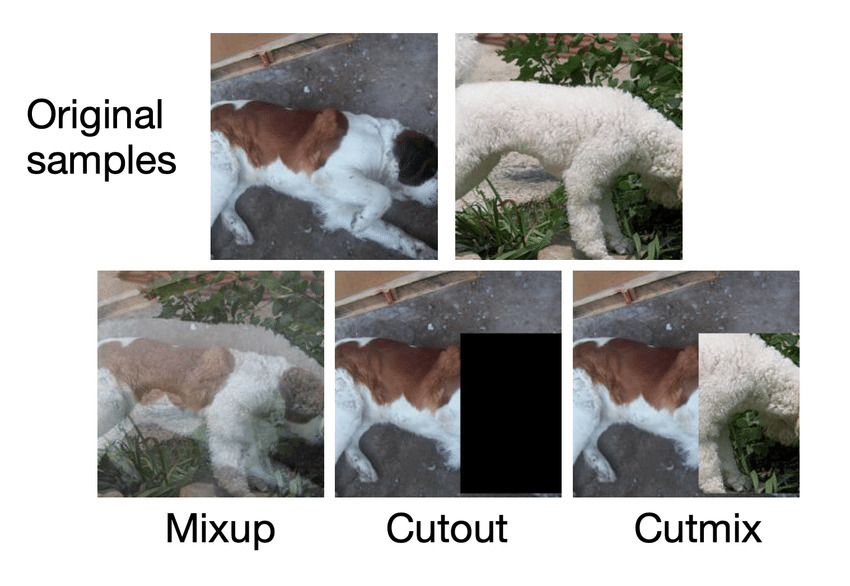
\includegraphics[scale=0.4]{Images/advanced-augmentation-methods.jpg}
    \caption{Advanced image augmentation examples~\cite{AdvAugExamples}.}
    \label{fig:advAugExamples}
\end{figure}

\section{Data Augmentation Using GANs}
\label{ssec:augmentationGANs}

In Section \ref{ssec:typesOfGANs}, the various types of Generative Adversarial Networks (GANs) were described. In this section, the focus will be on how GANs can help synthesize new, realistic data samples to expand existing datasets.

Generative Adversarial Networks (GANs) are leveraged for data augmentation by \textbf{synthesizing new, realistic data samples} that expand existing datasets. This capability is particularly valuable in fields where data collection is challenging or costly. GANs are sometimes described as a way to “unlock” additional information from a dataset. By generating diverse and high-quality artificial samples, GANs improve the robustness of machine learning models, helping them perform better in real-world applications by providing a richer and more varied training environment. Among the variety of GAN models, DCGANs, Conditional GANs, StyleGANs, and CycleGANs are particularly notable for their extensive potential in enhancing data augmentation efforts. 

\textbf{Conditional GANs}: cGANs are particularly useful for data augmentation in classification tasks by generating data samples conditioned on specific labels or attributes. By conditioning the generation process on specific labels, cGANs can produce diverse and representative samples across various classes, addressing \textbf{class imbalance} effectively.  For instance, in a scenario where certain classes are underrepresented, cGANs can generate additional samples for these classes, thereby improving the robustness of classification models. This targeted augmentation helps in achieving more accurate and generalizable classification outcomes in areas such as image recognition and medical diagnostics. For instance, cGANs were successfully used in this paper~\cite{cGANSAugmentation} for improving the Facial Emotion Recognition capabilities of the CNN.

\textbf{StyleGANs}: StyleGANs are particularly effective for data augmentation due to their ability to manipulate and refine \textbf{specific features} in images. This capability allows for the generation of varied data instances with controlled modifications to particular attributes, such as changing hairstyles, facial features, or expressions in human portraits. This targeted and high-quality augmentation can vastly improve the performance of classification. In the fashion industry, for instance, StyleGANs can create numerous variations of a clothing item in different colors and styles from a single base image, significantly expanding the dataset for training machine learning models aimed at fashion trend forecasting or recommendation systems. 

\textbf{CycleGANs}: CycleGANsare a particularly useful tool for data augmentation due to their ability to perform \textbf{image-to-image translations} without requiring paired examples. This unique ability makes them ideal for generating realistic variations of images across domains, such as converting summer landscapes to winter or turning photographs into paintings. A practical application of CycleGANs is in the training of autonomous vehicles, where they can simulate various weather conditions to help models learn to navigate under different environmental scenarios. Similarly, in medical imaging, they can alter healthy scans to exhibit pathological features, as seen in Figure \ref{fig:cycleGANBreastCancer}. This technique provides additional data for training diagnostic tools and can ultimately improve patient outcomes.

\begin{figure}[!htb]
    \centering
    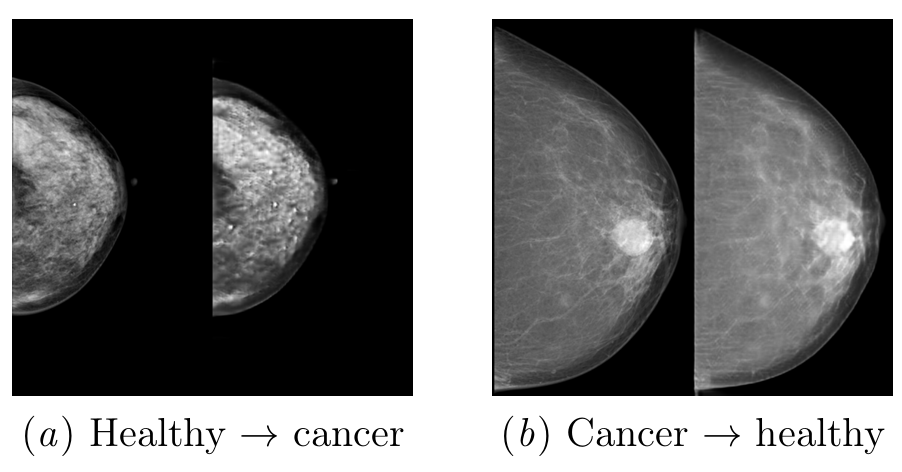
\includegraphics[scale=0.6]{Images/cycle-gan-breast-cancer.png}
    \caption{CycleGAN example -- transforming between breast cancer and healthy sample~\cite{CycleGANBreastCancer}.}
    \label{fig:cycleGANBreastCancer}
\end{figure}

\textbf{Data Augmentation Generative Adversarial Networks (DAGANs)}: DAGANs represent a significant advancement in GAN architecture, specifically aimed at enhancing data augmentation capabilities. Unlike traditional GANs, which generate new data points from random noise, DAGANs augment existing datasets by producing variations of the input data. This is accomplished by incorporating a U-Net-like structure into the generator architecture, enabling it to more accurately capture and reproduce variations within the context of the input data. Additionally, DAGANs implement an augmented adversarial training method technique that enhances the generator's ability to produce diverse, yet plausible, data variations. This makes them particularly useful for applications that require extensive and diverse training data from limited samples, such as one-shot learning.

When it comes to different GANs, \textbf{choosing the appropriate architecture} is crucial and depends on the dataset's specific needs and computational resources. DCGANs, Conditional GANs, StyleGANs, CycleGANs, and DAGANs each offer unique approaches for generating new, realistic data samples that significantly enhance data augmentation efforts. Each GAN type possesses distinctive features, such as managing class imbalances, adjusting particular image features, or converting images across diverse styles without the need for matching examples. Hence, selecting the most suitable GAN architecture requires careful consideration of what specific improvements are required and the computational capabilities available to ensure optimal machine learning model performance.

\begin{figure}[!htb]
    \centering
    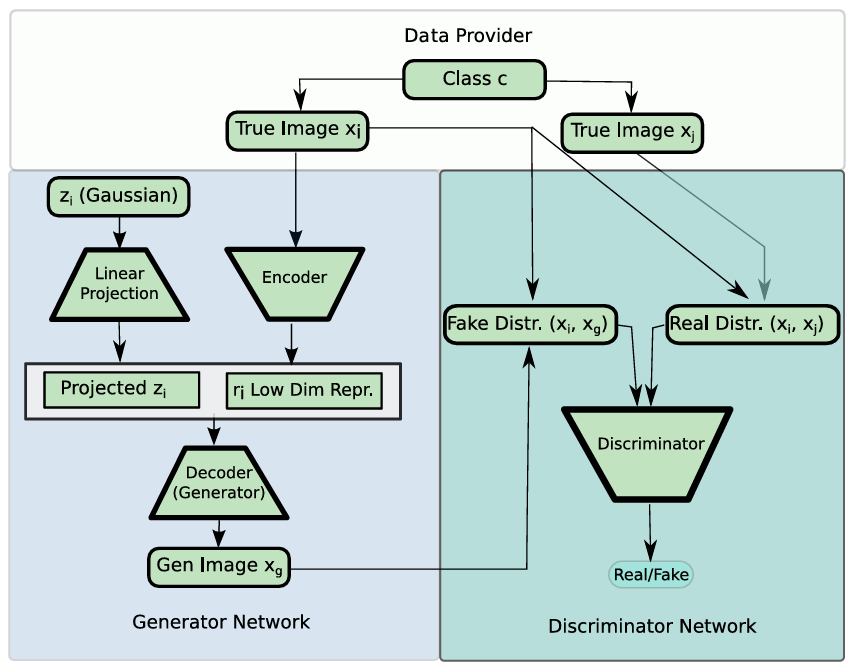
\includegraphics[scale=0.8]{Images/dagan-architecture.png}
    \caption{\textbf{DAGAN Architecture}. The image we want to use for augmentation is projected down to a lower dimensional representation and random noise is concatenated to this signal. This serves as an input to the generator and helps to limit variations of the input image, which is a valuable feature for image augmentation~\cite{DAGANPaper}.}
    \label{fig:DAGANArchitecture}
\end{figure}

%---------------------------------------------------------------------------

\section{Domain Specific Audio Augmentation}
\label{ssec:domainSpecific}

This section of the thesis analyzes the significance of Mel Spectrograms and their role in transforming audio signals into image-based formats for analytical purposes. Various approaches to enhancing raw audio and custom techniques for augmenting spectrogram representations are explored. These methods enhance datasets for training deep learning models in sound analysis.

\subsection{Mel Spectrograms}
\textbf{Mel Spectrograms} are visual representations of audio files created by converting audio signals into the frequency domain using the Short-Time Fourier Transform (STFT). The STFT splits the signal into short segments and computes the Fourier transform for each, resulting in a two-dimensional array representing time and frequency. These frequencies are then converted to the Mel scale, which mimics human pitch perception, using a series of triangular overlapping filters.

Mel Spectrograms allow audio file classification to be treated like image classification, enabling the use of techniques such as convolutional neural networks (CNNs). Advantages of using Mel Spectrograms include:
\begin{itemize}
   \item \textbf{Dimensionality Reduction}: For a 30-second audio file sampled at a frequency of $22,050$ Hz, dimensionality reduction can decrease the number of input parameters by a factor of $10$, from $[1, 661, 500]$ to $[64, 1024]$.
   \item Mel spectrograms map audio signals to a frequency scale that reflects \textbf{human hearing}, making them more relatable and intuitive for tasks involving human sound perception.
   \item Mel spectrograms simplify the \textbf{audio patterns extraction}, aligning with the way CNNs identify patterns in images, allowing for more effective audio recognition.
   \item \textbf{Robustness to noise} and variations.
   \item Enable sound to be analyzed using \textbf{image-processing techniques}.
\end{itemize}

While some augmentations are best applied directly to the raw audio signal, others are more suited to the spectrogram format.  Figure \ref{fig:audioAugDiagram} provides a visualization of this concept.

\begin{figure}[!htb]
    \centering
    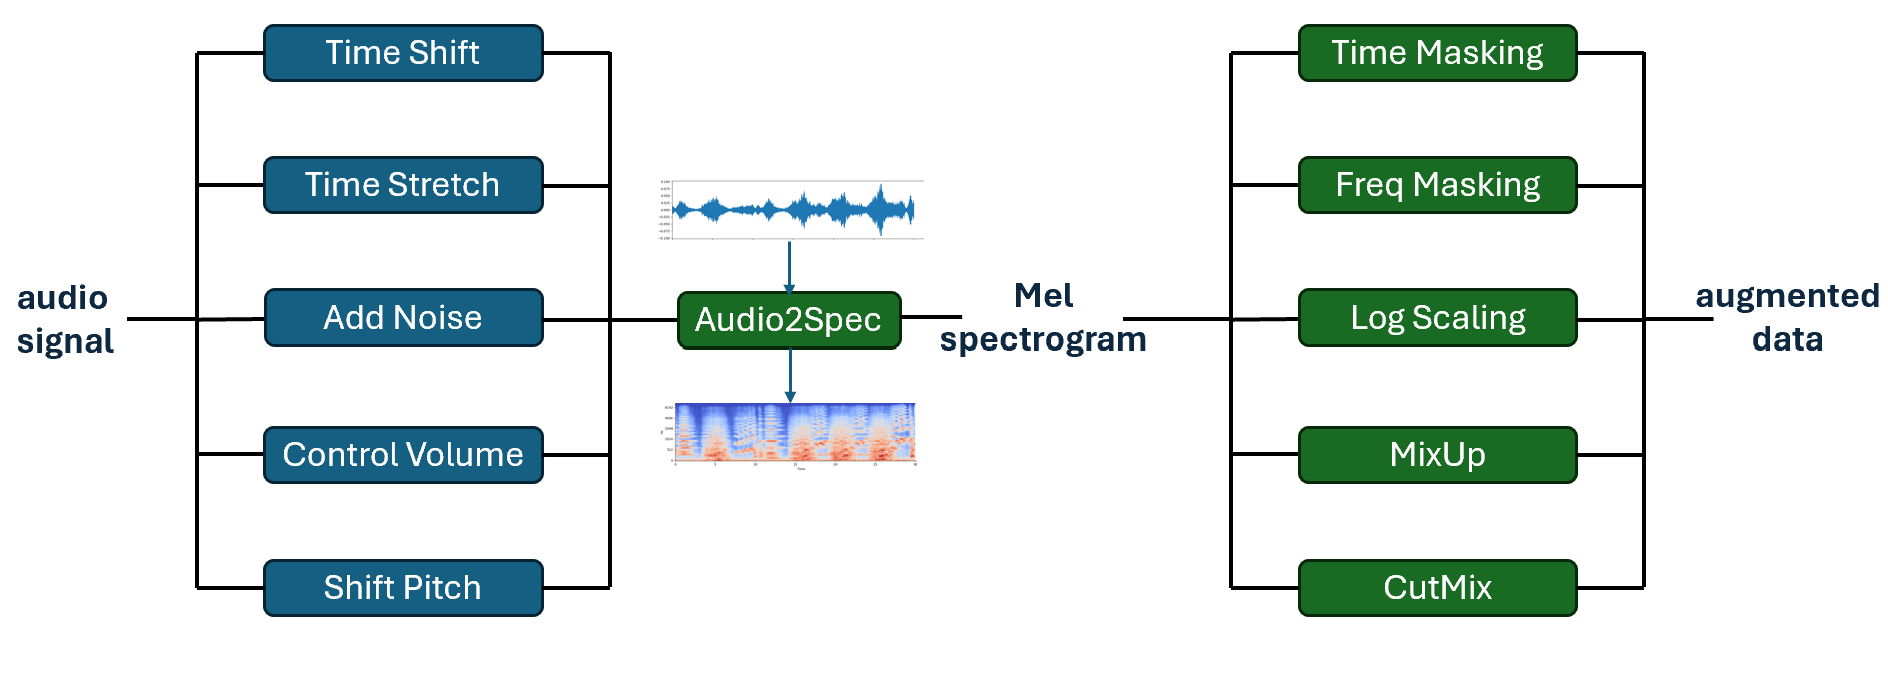
\includegraphics[scale=0.58]{Images/audio-augmentation.png}
    \caption{Audio Augmentation diagram.}
    \label{fig:audioAugDiagram}
\end{figure}

\subsection{Audio Signal Augmentation}

This section of the thesis is based on the article "Data Augmentation and Deep Learning Methods in Sound Classification: A Systematic Review"~\cite{AudioAugmentation}.

\textbf{Time Shifting} is an augmentation technique, where an audio sample is delayed or advanced in time. The utility of this method lies in its ability to simulate the real-world scenario where sounds may not always start at the same temporal threshold, which helps the model handle these events effectively.

\textbf{Time Stretching} manipulates the time dimension of the sound wave without altering its pitch. This technique teaches models that variations in playback speed and duration of audio events can occur. That is particularly beneficial in voice recognition systems where speaker cadences vary widely.

\textbf{Adding Noise} is a universal method in audio augmentation, imitating the presence of ambient noise in everyday soundscapes. By blending signals with a range of noise types, models are trained to extract relevant audio features even when masked by background interference. Test data is often collected in noisier environments, requiring models to effectively manage and adapt to these challenges.

\textbf{Volume Control} serves as another augmentation strategy, which adjusts the amplitude of audio signals. This method teaches models to determine audio patterns across different decibel levels, mitigating the model's sensitivity to volume variations that can affect the clarity of sounds in practical applications.

\textbf{Pitch Shifting} involves changing the pitch of audio signals to mimic the natural pitch variations in human speech and musical instruments. This technique is crucial for models designed for speech-processing tasks and music genre classification, where pitch plays a significant role in conveying meaning.

\begin{figure}[!htb]
    \centering
    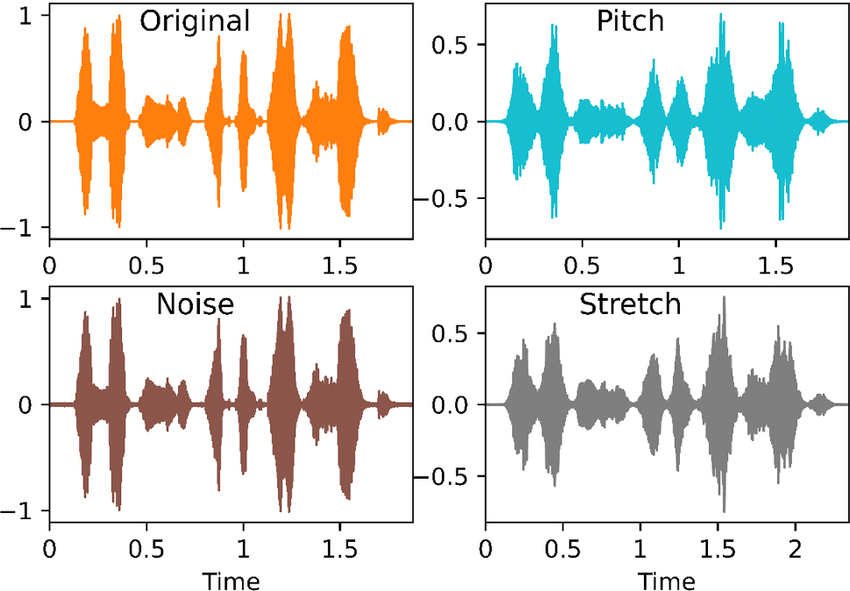
\includegraphics[scale=1.2]{Images/raw-audio-augmentations.png}
    \caption{Audio signal augmentation examples~\cite{RawAudioAugmentation}.}
    \label{fig:rawAudioAugmentation}
\end{figure}

\subsection{Spectrogram Based Augmentation}

The first method is called \textbf{Time Masking}. It involves hiding sequential time steps in the Mel spectrogram, similar to slicing away a vertical strip from an image. This forces learning algorithms to interpolate missing temporal information, improving resilience to temporal distortions, omissions, or differences in real-world audio. The width and number of strips can be adjusted using function parameters.

\textbf{Frequency Masking} is similar to time masking but targets the frequency axis, hiding horizontal stripes to mask a range of frequencies. This simulates frequency loss, crucial for training models to perform well even when certain frequency bands are missing or damaged, a common occurrence in various acoustic environments.


\textbf{Log Scaling}, is another method that involves applying a logarithmic function to the frequency domain. This enhances the detail in lower frequencies and brings the spectrogram's representation closer to human hearing perception.

\textbf{MixUp} in audio blends two different audio clips and their corresponding labels to create a new sample. This process merges the audio signals and computes a weighted average of their labels. For example, combining "people talking" and "guitar playing" clips results in a new audio clip and label reflecting this mix, based on a lambda parameter. This encourages the model to learn from mixed audio scenarios, enhancing its ability to handle uncertainty and overlapping sounds common in real-world conditions.

\textbf{CutMix} in audio slices a segment from one audio spectrogram and pastes it onto another, creating a composite spectrogram. Unlike \textit{MixUp}, which uniformly blends audio, \textit{CutMix} forces the model to make predictions from incomplete or obscured sounds, as the pasted segment may hide key features of the base audio. This technique improves the model's performance in scenarios where parts of a song might suggest a different musical genre than the song as a whole.

\begin{figure}[!htb]
    \centering
    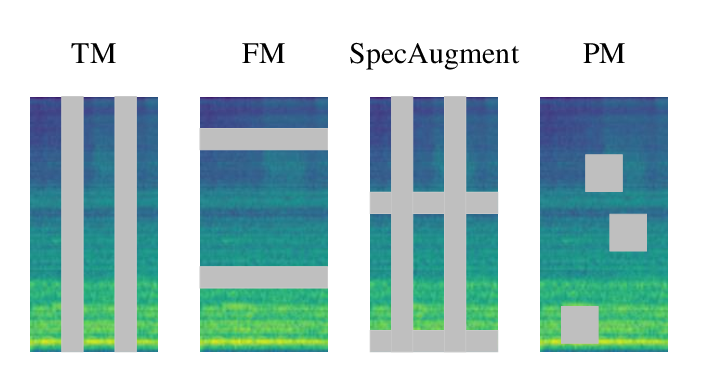
\includegraphics[scale=0.8]{Images/spectrogram-masking.png}
    \caption{Spectrogram-based augmentation example~\cite{MaskingAugmentation}.}
    \label{fig:specAudioAugmentation}
\end{figure}

\section{Data Augmentation Safety}

In the context of data augmentation techniques, it is essential to recognize both their benefits and potential drawbacks to ensure that they improve model performance instead of undermining it. This section of the thesis considers the risks associated with various common augmentation strategies and highlights the importance of careful implementation.

\textbf{Rotation} and \textbf{flipping} are widely used for augmenting image data. However, these methods can introduce significant distortions if not appropriately applied. For instance, arbitrary rotation of images such as flowers can lead a model to learn incorrect orientations since flowers in nature do not exhibit a full 360-degree rotational symmetry. Similarly, horizontally flipping text data can create nonsensical sequences, making it challenging to analyze documents with natural language processing.

\textbf{Cropping} and \textbf{shifting} are another commonly employed techniques that, while useful in focusing a model's attention on salient image features, can also remove essential parts of an image. In scenarios where important features are cropped out, the model may learn from incomplete or irrelevant data, leading to poor performance. This is particularly critical in applications like facial recognition, where missing features such as eyes or mouths can severely impact the model's accuracy.

The use of \textbf{Generative Adversarial Networks} (GANs) introduces a different set of challenges. While GANs are powerful in generating new, synthetic images, they can produce data that does not represent any real-world distribution if not carefully tuned. This can lead to models that perform well on synthetic data but poorly on actual data.

\textbf{Mixing images} can also lead to confusion. If only a small, yet crucial, part of an image is used and overlaid by a less relevant part of another image, it can mislead the model about the importance and context of the features.

In the field of \textbf{medical image analysis}, improper geometric or color transformations can distort anatomical details and critical color information, potentially leading to incorrect diagnoses. For example, overly darkening an image can obscure important details, while removing red can hide signs of bleeding.

These examples highlight the need for careful planning and evaluation when implementing data augmentation techniques. It is crucial to understand the specific characteristics and requirements of the data to ensure that augmentation methods are enhancing the training process and not introducing misleading biases. Such considerations are vital for developing robust machine learning models that are reliable and effective in real-world applications.